\section{Wet/dry Interface}

The numerical solvers can yield spurious negative water depth. This non-physical phenomena can occur mainly during the wetting and drying processes in the computational domain as shown in Figure \ref{wetDry}. This phenomena is well known from the theory of finite volumes \cite{audusse, Audusse2005, cotoJe, Casulli2009, 
Fiser2014, Hou2013, Hou2014, Kesserwani2013, Medeiros2013}. In \cite{kurg2}, Kurganov et al. suggested positivity preserving scheme based on finite volume method. This scheme modifies the slope of linear reconstruction so that there is no negative water depth within the finite volume.

 An exemplary finite volume reconstruction resulting in negative water depth 
at the edge $i-\frac12$ is shown in Figure \ref{negW}. The negative 
water depth $h_{i-\frac12}$ at the edge $i-\frac12$ is set to zero and the water 
depth $h_{i+\frac12}$ is computed in such way that the water depth at cell center 
$h_i$ remains unchanged:
\begin{equation}
\begin{array}{c}
\underbrace{0}_{h_{i-\frac12}}+B_{i-\frac12}+\delta h_i \frac{\Delta x_i}{2}=
h_i+\frac{B_{i+\frac12}+B_{i-\frac12}}{2}\\
\Downarrow\\
\delta h_i=\frac{2h_i+B_{i+\frac12}-B_{i-\frac12}}{\Delta x_i}
\end{array}
\end{equation}
Here $\delta h_i$ is the slope of the water level. Then 
\begin{equation}
h_{i+\frac12}=h_i+\frac{B_{i+\frac12}+B_{i-\frac12}}{2}+
\delta h_i \frac{\Delta x_i}{2}-B_{i+\frac12}=2h_i.
\end{equation}
The corrected reconstruction of the water depth is shown in 
Figure \ref{zeroW}.
\begin{figure}[t]
\centering
\begin{minipage}[t]{0.44\textwidth}
\begin{center}
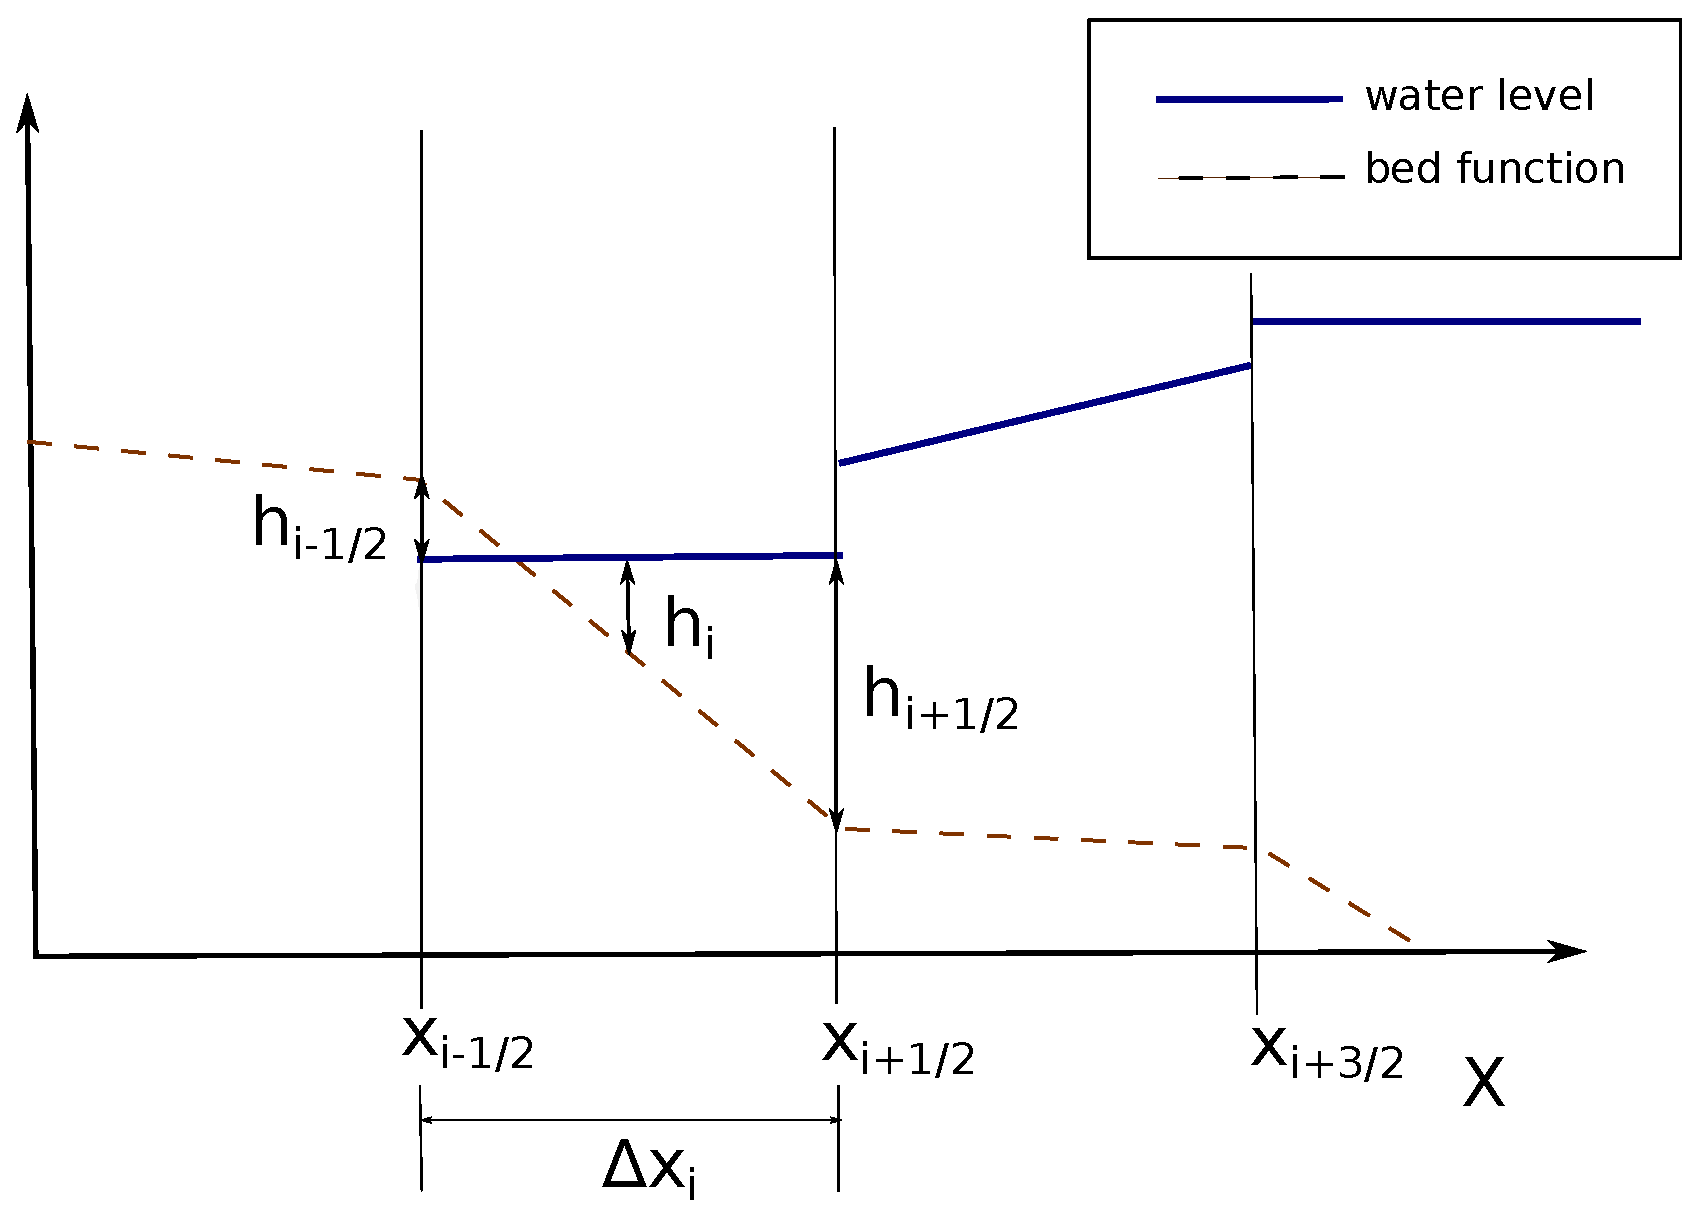
\includegraphics[width=1\textwidth]{OBR/negW.eps}
\caption{Linear reconstruction of the water depth with the negative water depth $h_{i-\frac12}$.}\label{negW}
\end{center}
\end{minipage}\hspace{15mm}
\begin{minipage}[t]{0.44\textwidth}
\begin{center}
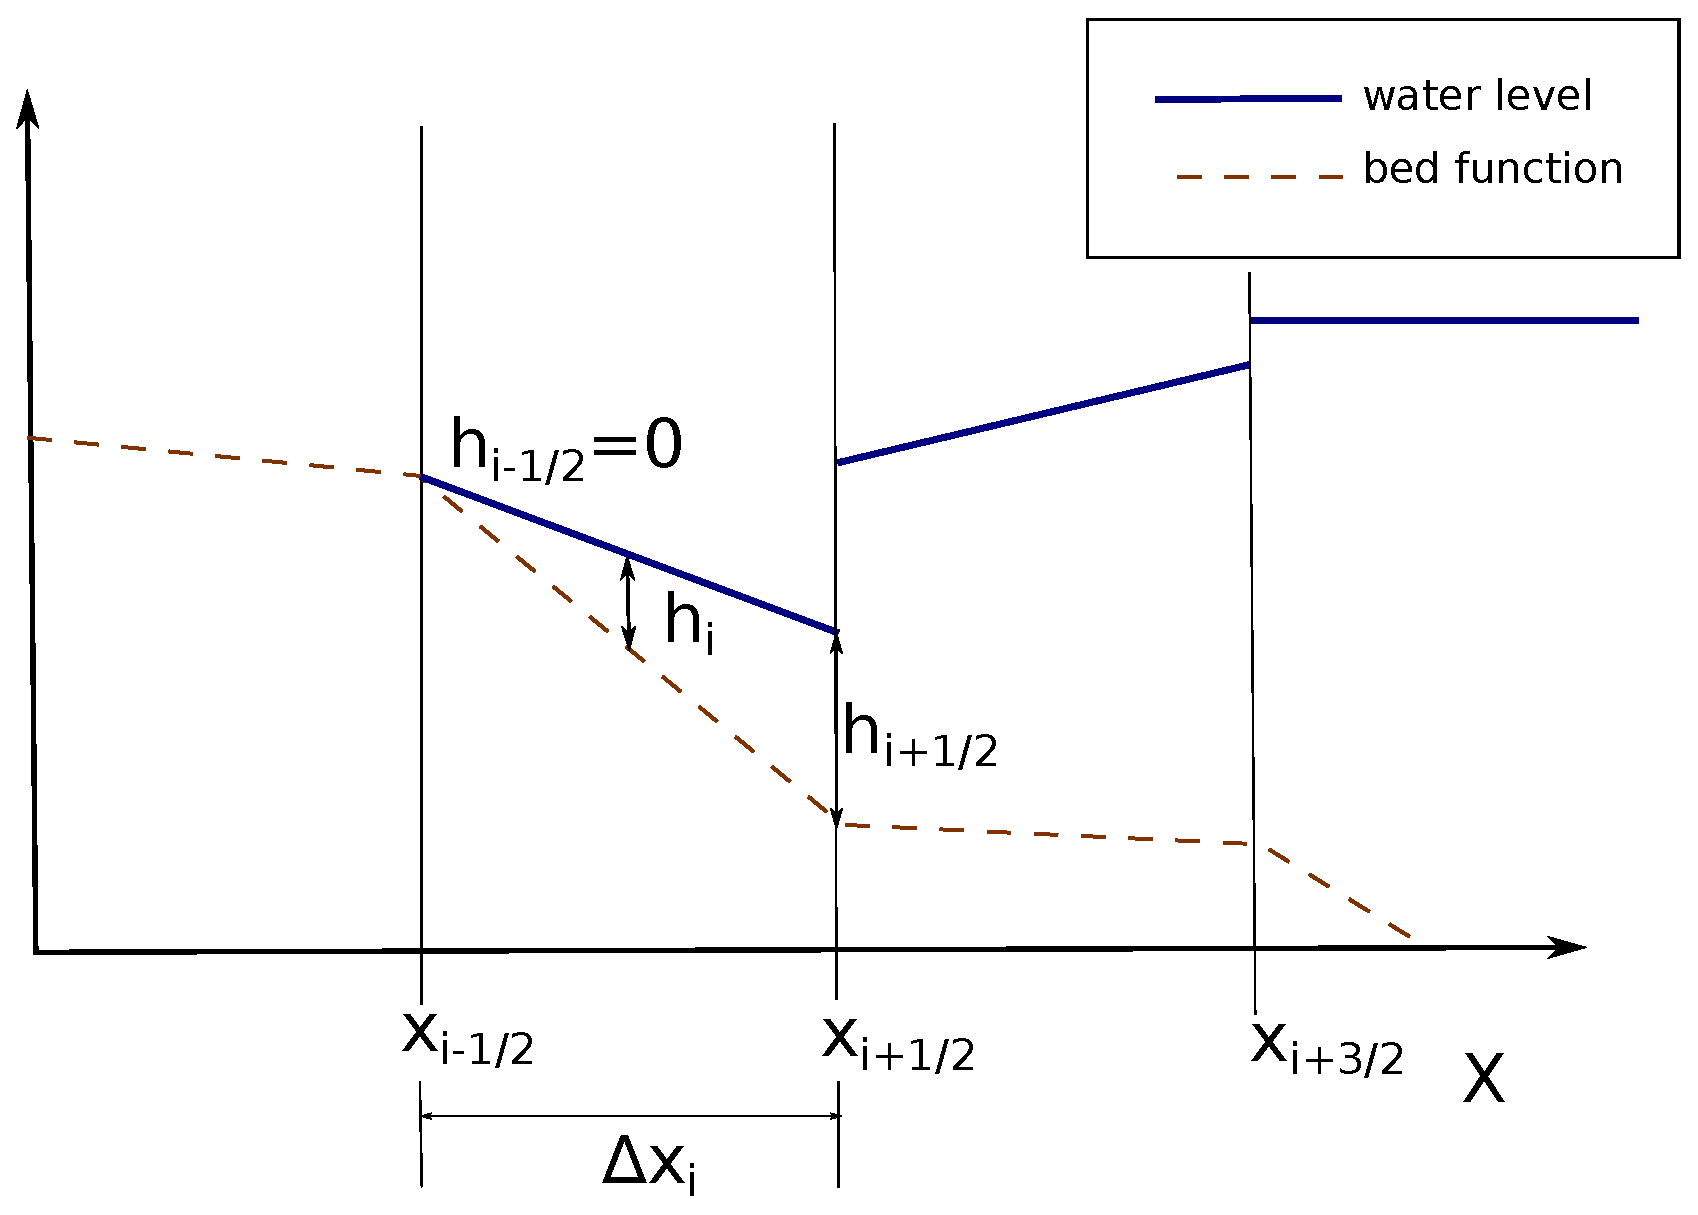
\includegraphics[width=1\textwidth]{OBR/zeroW}
\caption{Corrected linear reconstruction of the water depth.}\label{zeroW}
\end{center}
\end{minipage}
\end{figure}	
The case when $h_{i+\frac12}<0$ can be corrected in a similar way and the conditions of the 
correction can be summarized as \cite{kurg2}
\begin{equation}\label{kurgMod}
\begin{array}{c}
\text{if} \quad h_{i-\frac12}<0 \begin{cases}
h_{i-\frac12}=0\\
h_{i+\frac12}=2h_i
\end{cases},\\
\\
\text{if} \quad h_{i+\frac12}<0 \begin{cases}
h_{i-\frac12}=2h_i\\
h_{i+\frac12}=0
\end{cases}.\\
\end{array}  
\end{equation}
After this modification, the non-negativity of the water depth is ensured. 

Higher order DGFEM method can produce the negative values of the water depth not only at the edges but also within the finite element as shown in Figure \ref{wetDry}.
\begin{figure}
\centering
\includegraphics[width=0.7\textwidth]{OBR/wetDry.eps}
\caption{Non-physical solution with negative water depth.}\label{wetDry}
\end{figure}
 It is computationally demanding to check whole solution within the finite element thus we suggest to check the positivity of the solution only in the points which are used for the computations. These points are the Gaussian points and values at the edges of the finite element. This process results in novel criterion for wet/dry interface. The solution must be limited if 
 \begin{equation}
 W_{i,1}(x_p)<0
 \end{equation}
where $x_p$ stands for Gaussian points and points at the edges of the finite element. First part of the limitation of the water depth is similar to that one described in Section \ref{limSec}. The third coefficient is set to be zero which yields the situation depicted in Figure \ref{lin}. 
\begin{figure}
\centering
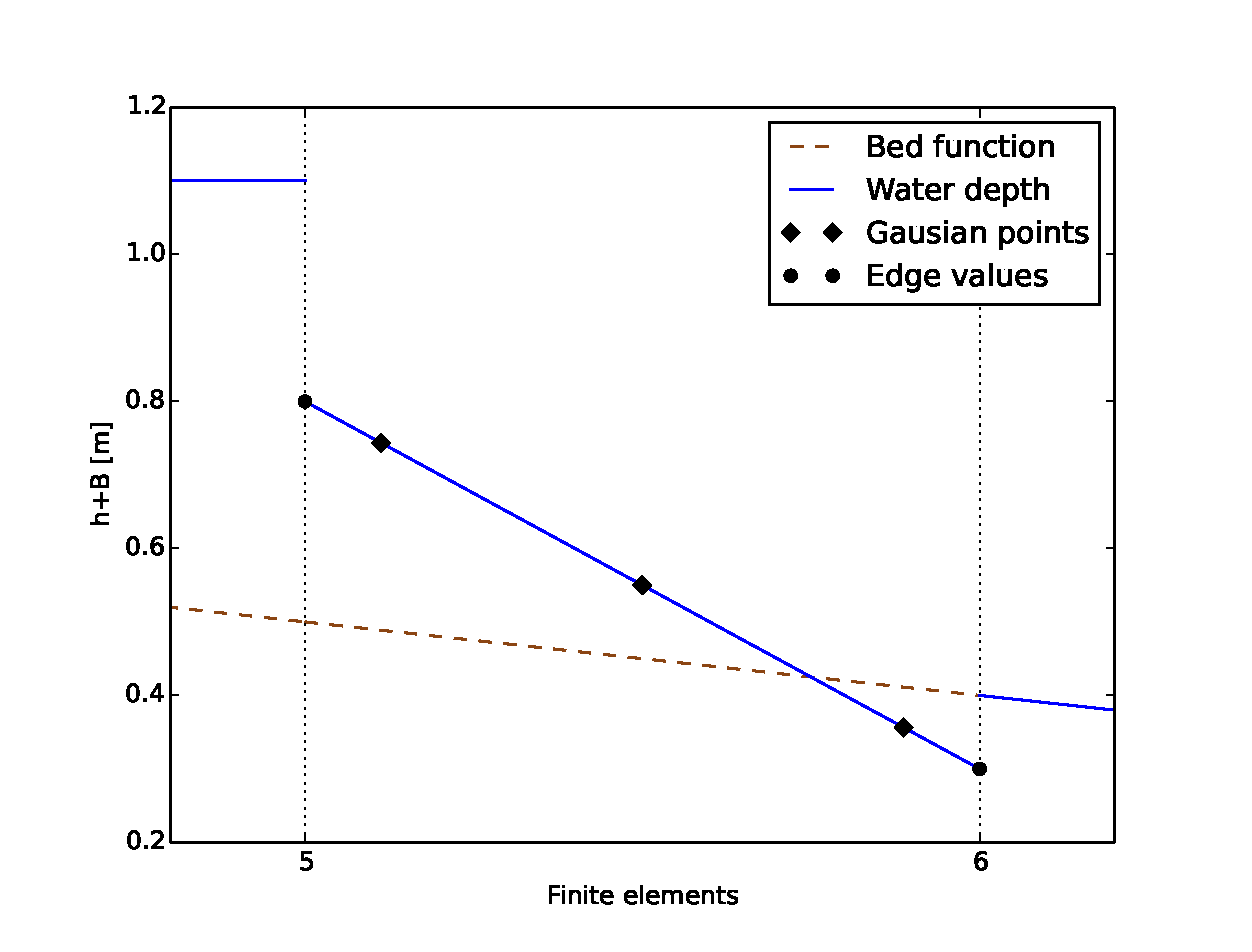
\includegraphics[width=0.7\textwidth]{OBR/lin.eps}
\caption{Limited solution of the water depth.}\label{lin}
\end{figure}
After that, the coefficient $w_{i,1}^2$, governing the slope of the linear function, is altered to gain the same values as in (\ref{kurgMod}). It means that, in case when the water depth $W_{i,1}(x_{i-\frac12})$ is negative, the slope of the function can be computed as
\begin{equation}\label{slope}
w_{i,1}^2=\frac{W_{i,1}(x_{i})-0}{ \frac{\Delta x_i}2}=W_{i,1}(x_{i}).
\end{equation}
Let us highlight that $\Delta x_i=2$ because of the mapping (\ref{mapping}) and after the limitation to the linear function, the value of the water depth in the middle of the finite element is equal to the first coefficient, i.e.
\begin{equation}\label{coefVal}
W_{i,1}(x_{i})=w_{i,1}^1.
\end{equation}
 Taking in account (\ref{coefVal}), relation (\ref{slope}) can be generalised for both edges as
\begin{equation}
w_{i,1}^2=\begin{cases}
w_{i,1}^1, \text{  if  } W_{i,1}(x_{i-\frac12})<0 \\
-w_{i,1}^1, \text{  if  } W_{i,1}(x_{i+\frac12})<0
\end{cases}.\\
\end{equation}
Final limited and corrected solution can be seen in Figure \ref{linCor}.
\begin{figure}
\centering
\includegraphics[width=0.7\textwidth]{OBR/linCor.eps}
\caption{Corrected solution of the water depth.}\label{linCor}
\end{figure}




However this water depth may become very small and cause problems with the computation of 
the velocity $u$ which is computed by the fraction of the discharge ($hu$) and water depth $h$ 
\begin{equation}
u=\frac{(hu)}{h}. 
\end{equation}
Obviously $u\rightarrow\infty$ for $h\rightarrow 0$. To avoid unrealistic velocities, 
Kurganov and Petrova \cite{kurg2} proposed the following formulae which 
avoids the division by very small numbers
\begin{equation}\label{formVel}
u=\frac{\sqrt{2}h(hu)}{\sqrt{h^4+\max(h,\epsilon_h)}}.
\end{equation}
$\epsilon_h$ is a small positive constant. In \cite{kurg2} it is 
recommended to set this constant to $\epsilon_h=(\Delta x_i)^4$.
The discharge $hu$, used in the Riemann solver, has to be recomputed as
\begin{equation}
hu=h\cdot u.
\end{equation}

